\subsection{Rocket flight physics model}
\label{subsec:rocket_flight_model}

To compute a simple flight dynamics model, it's necessary to observe the force acting on the rocket.
In Figure \ref{fig:forces_on_rocket}, the rocket is represented by a rectangle, and the forces acting on it are shown.

\begin{figure}[H]

    \centering
    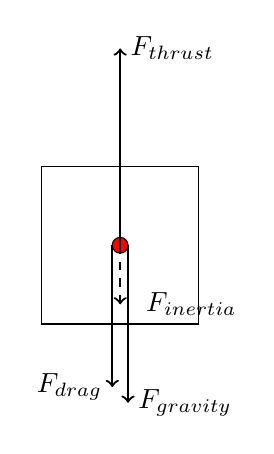
\begin{tikzpicture}

        \draw (0,0) rectangle (2, 2);

        \filldraw[fill=red, draw=black] (1, 1) circle (0.1);

        \draw[thick, ->] (1-0.1, 1) -- ++(0, -1.8) node[left] {$F_{\text{drag}}$};
        \draw[thick, ->] (1+0.1, 1) -- ++(0, -2) node[right] {$F_{\text{gravity}}$};
        \draw[thick, ->] (1, 1) -- ++(0, +2.5) node[right] {$F_{\text{thrust}}$};
        \draw[thick, ->, dashed] (1, 1) -- ++(0, -0.75) node[right=0.2cm] {$F_{\text{inertia}}$};

    \end{tikzpicture}
    \caption{Forces acting on the rocket during the flight.}
    \label{fig:forces_on_rocket}

\end{figure}

A simple balance of forces can be written as:

\begin{equation}
    F_{\text{thrust}} - F_{\text{drag}} - F_{\text{gravity}} = F_{\text{inertia}}
\end{equation}


\paragraph{Thrust force}

$F_{\text{thrust}}$ is the thrust force that the engine is supposed to deliver to the rocket during its flight.
In particular, knowing that the engine used for the rocket is a \texttt{TSP F35} engine, we can retrieve the thrust curve from the manufacturer's website obtaining the data shown in Figure \ref{fig:thrust_curve}.

\begin{figure}[H]
    \centering
    \includegraphics[width=.6\textwidth]{img/Thrust_curve.png}
    \caption{Thrust curve of the \texttt{TSP F35} engine.}
    \label{fig:thrust_curve}
\end{figure}

Equivalently, the thrust points are reported in Table \ref{tab:thrust_points}.

\begin{table}[H]
    \centering
    \begin{tabular}{|c|c|}
        \hline
        \textbf{Time [s]} & \textbf{Thrust [N]} \\
        \hline
        $0.000$           & $0.000$             \\
        $0.090$           & $34.235$            \\
        $0.155$           & $49.765$            \\
        $0.203$           & $54.706$            \\
        $0.262$           & $50.118$            \\
        $0.393$           & $32.118$            \\
        $0.603$           & $33.529$            \\
        $0.795$           & $31.059$            \\
        $0.999$           & $30.706$            \\
        $1.205$           & $30.000$            \\
        $1.408$           & $29.647$            \\
        $1.608$           & $29.647$            \\
        $1.801$           & $27.882$            \\
        $1.997$           & $28.235$            \\
        $2.042$           & $24.706$            \\
        $2.118$           & $8.471$             \\
        $2.197$           & $0.000$             \\
        \hline
    \end{tabular}
    \caption{Thrust points of the \texttt{TSP F35} engine.}
    \label{tab:thrust_points}
\end{table}

Given that we are going to solve the system at time step much more smaller than the time step of the thrust curve, we can interpolate the thrust curve to obtain the thrust force at each time step.

In the end, we can write:

\begin{equation}
    F_{\text{thrust}} = F_{\text{thrust}}(t_i) \approx F_{\text{thrust, interpolated}}(t)
\end{equation}


\paragraph{Drag force}

$F_{\text{drag}}$ is the drag force acting on the rocket during the flight.
This force can be computed as:

\begin{equation}
    F_{\text{drag}} = \frac{1}{2} \rho v^2 A C_d
\end{equation}

However, to more precise, we can also take into account some non-linearity of the equation such as the variation of the air density with respect to the altitude $\rho(\tilde{z})$ (see Equation \ref{eq:atmospheric_pressure}).
If this is the case, then the drag force can be computed as:

\begin{equation}
    F_{\text{drag}} = F_{\text{drag}}(\tilde{z}, v) = \frac{1}{2} \rho(\tilde{z}) v^2 A C_d
\end{equation}


\paragraph{Gravity force}

$F_{\text{gravity}}$ is the gravity force acting on the rocket during the flight.
This force can be computed as:

\begin{equation}
    F_{\text{gravity}} = m g
\end{equation}

However, it's important to notice that the mass of the rocket is not constant during the flight, but it's decreasing due to the fuel consumption.
In particular, knowing that the mass of the rocket at the beginning and at the end of the flight is $m_0 = 0.316kg$ and $m_f = 0.224kg$ respectively, we can compute the mass of the rocket function of time as:

\begin{equation}
    m(t) = \begin{cases}
        m_0 - \frac{m_0 - m_f}{t_f} t & \text{if } t \leq t_f \\
        m_f                           & \text{if } t > t_f
    \end{cases}
\end{equation}

Where $t_f$ is the time at which the engine stops working (see last row of Table \ref{tab:thrust_points}).

By doing so, the gravity force can be computed (neglecting any variation of the gravity with respect to the altitude) as:

\begin{equation}
    F_{\text{gravity}} = F_{\text{gravity}}(t) = m(t) g
\end{equation}


\paragraph{Inertia force}

$F_{\text{inertia}}$ is the inertia force acting on the rocket during the flight.
This force can be computed as:

\begin{equation}
    F_{\text{inertia}} = m(t) a(t)
\end{equation}

Where $a(t)$ is the acceleration of the rocket at time $t$.

